\documentclass{beamer}


\mode<presentation> {

% The Beamer class comes with a number of default slide themes
% which change the colors and layouts of slides. Below this is a list
% of all the themes, uncomment each in turn to see what they look like.

% \usetheme{default}
\usepackage{bookman}
\usetheme{Madrid}
\usefonttheme{serif}
\usecolortheme{beaver}
\setbeamertemplate{theorems}[numbered] 
\setbeamertemplate{navigation symbols}{}
\setbeamertemplate{frametitle}[default][center]
}

\usepackage[many]{tcolorbox}
\usepackage{graphicx} % Allows including images
\usepackage{booktabs} % Allows the use of \toprule, \midrule and \bottomrule in tables
\usepackage{amsmath,amsfonts,amssymb,mathtools,derivative,systeme,hyperref,relsize,graphicx,ulem}
\usepackage{stmaryrd}
\usepackage{xspace}
\usepackage{pgfplots}
\usetikzlibrary{patterns,positioning,arrows.meta,shapes.geometric,calc}
\pgfplotsset{compat=1.18}
% \usefonttheme[onlymath]{serif}
\newcommand{\Mod}[1]{\ (\mathrm{mod}\ #1)}
\newcommand{\tendsto}[1]{%
    \xrightarrow{\smash{\raisebox{-2ex}{$\scriptstyle#1$}}}}

% \newcommand{\verifier}{\color{orange}}
\newcommand{\setup}{\color{blue}}
% \newcommand{\eval}{\color{red}}
\newcommand{\verifierc}{orange}
\newcommand{\setupc}{blue}
\newcommand{\evalc}{red}
\providecommand{\false}{\ensuremath{\mathsf{false}}}
\providecommand{\true}{\ensuremath{\mathsf{true}}}
\providecommand{\pcto}{\ensuremath{\mathsf{to}}}
\providecommand{\pcpos}{\ensuremath{\mathsf{at}}}
\providecommand{\pcrow}{\ensuremath{\mathsf{row}}}
\providecommand{\pcrows}{\ensuremath{\mathsf{rows}}}
\providecommand{\pcrowsize}{\ensuremath{\mathsf{getRowSize}}}
\providecommand{\pccase}{\ensuremath{\mathbf{case}}\ }
\providecommand{\pcswitch}{\ensuremath{\mathbf{switch}}\ }
\providecommand{\breakalg}{\ensuremath{\mathsf{break}}}
\providecommand{\pcof}{\ensuremath{\mathbf{of}}\xspace}
\providecommand{\pcbreak}{\ensuremath{\mathbf{break}}\xspace}
\providecommand{\myprotocol}{\ensuremath{{\bf \Pi}}\xspace}
\providecommand{\toSV}{\ensuremath{{\tt to}\_{\tt SVSV}}\xspace}

\newcommand{\A}{\mathcal{A}}
\newcommand{\matrixA}{\ensuremath{\mathbf{A}}\xspace}
\newcommand{\matrixB}{\ensuremath{\mathbf{B}}\xspace}
\newcommand{\F}{\mathbb{F}}
\providecommand{\Group}{\mathbb{G}}
\newcommand{\N}{\mathbb {N}}
\newcommand{\Q}{\mathbb{Q}}
\newcommand{\Server}{\ensuremath{\mathcal{S}}\xspace}
\newcommand{\T}{\ensuremath{{\tt T}}}
\newcommand{\Z}{\mathbb {Z}}
\newcommand{\He}{\mathcal{H}}
\newcommand{\id}{{\sf id}}

\newcommand{\FF}{\ensuremath{\mathbb F}}
\newcommand{\fp}{\ensuremath{\FF_p}}
\newcommand{\fps}{\ensuremath{\FF_p^*} }
\newcommand{\fpk}{\ensuremath{\FF_{p^k} } }
\newcommand{\fpks}{\ensuremath{\FF_{p^k}^*}}
\newcommand{\fq}{\ensuremath{\FF_q}}
\newcommand{\fqk}{\ensuremath{\FF_{q^k}}}
\newcommand{\fqks}{\ensuremath{\FF^*_{q^k}}}
\newcommand{\fpt}{\ensuremath{\FF_{p^2}}}
\newcommand{\fpts}{\ensuremath{\FF_{p^2}^*}}
\providecommand{\Mod}[1]{\ (\mathrm{mod}\ #1)}

\newcommand{\xdownarrow}[1]{%
  {\left\downarrow\vbox to #1{}\right.\kern-\nulldelimiterspace}
}

%%%%%%%%%%%%
%% ALGORITHMS
%%%%%%%%%%%%
\providecommand{\enc}{\ensuremath{{\sf ENC}}\xspace}
\providecommand{\dec}{\ensuremath{{\sf DEC}}\xspace}
\providecommand{\amore}{\ensuremath{\text{KAPR25}}\xspace}
\providecommand{\love}{\ensuremath{{\sf LOVE}}\xspace}
\providecommand{\keygen}{\ensuremath{{\sf KeyGen}}\xspace}
\providecommand{\probgen}{\ensuremath{{\sf ProbGen}}\xspace}
\providecommand{\compute}{\ensuremath{{\sf Compute}}\xspace}
\providecommand{\verify}{\ensuremath{{\sf Verify}}\xspace}
\providecommand{\onverify}{\ensuremath{{\sf Verify}}\xspace}
\providecommand{\onsetup}{\ensuremath{{\sf Setup}}\xspace}
\providecommand{\offsetup}{\ensuremath{{\sf OneTimeSetup}}\xspace}
\providecommand{\precompute}{\ensuremath{{\sf PreCompute}}\xspace}
\providecommand{\preco}{\hyperref[fig:amore]{\ensuremath{{\sf PreComp}}}\xspace}
\providecommand{\client}{\ensuremath{{\sf client}}\xspace}
\providecommand{\server}{\ensuremath{{\sf server}}\xspace}
\providecommand{\gsetup}{\ensuremath{{\sf GlobalSetup}}\xspace}
\providecommand{\init}{\ensuremath{{\sf InitState}}\xspace}
\providecommand{\bool}{} %\ensuremath{{\tt Bool}}\xspace}
\providecommand{\tstart}{\ensuremath{{\tt t}_{\sf start}}\xspace}
\providecommand{\tnow}{\ensuremath{{\tt time}.{\tt now()}}\xspace}
\providecommand{\devicebound}{\ensuremath{{\mathcal{B}}}\xspace}
%%%%%%%%%%%%
%% INPUTS
%%%%%%%%%%%%
\providecommand{\secpar}{\ensuremath{{\lambda}}\xspace}
\providecommand{\effpar}{\ensuremath{\varphi}\xspace}
\providecommand{\auxsecpar}{\ensuremath{ {\tt aux.sec}}\xspace}
\providecommand{\statsecpar}{\ensuremath{\sigma}\xspace}
\providecommand{\timepar}{\ensuremath{\tau}\xspace}
\providecommand{\roundpar}{\ensuremath{\kappa}\xspace}
\providecommand{\sk}{\ensuremath{{\sf sk}}\xspace}
\providecommand{\pk}{\ensuremath{{\sf pk}}\xspace}
\providecommand{\myinput}{\ensuremath{(A,B)}\xspace} %input to the outsourced computation
\providecommand{\serveroutput}{\ensuremath{{\tt out}}\xspace} %encoded output by the server
\providecommand{\secvalue}{\ensuremath{{\tt sec}}\xspace} %secret output of the client
\providecommand{\secarray}{\ensuremath{{\bf sec}}\xspace}
\providecommand{\pubvalue}{\ensuremath{{\tt pub}}\xspace} %public output of the client
\providecommand{\privvalue}{\ensuremath{{\tt priv}}\xspace} %private superscript in sec experiment
\providecommand{\state}{\ensuremath{{\tt sk}}\xspace} %state
\providecommand{\advstate}{\ensuremath{{\tt st}}\xspace} %state
\providecommand{\offvalue}{\ensuremath{{\tt off}}\xspace} %public output of the client
\providecommand{\gpp}{\ensuremath{{\tt pp}}\xspace} %public parameters
\providecommand{\myresult}{{\ensuremath{\tt result}}\xspace} %encoded output by the server
\providecommand{\myresults}{{\ensuremath{\sf values}}\xspace}
\providecommand{\gp}{\ensuremath{{\sf gp}}\xspace}%globabl public parameters, crs
\providecommand{\pick}{\ensuremath{\overset{\,\$}{\gets}}\xspace}
\providecommand{\pickwithdist}{\ensuremath{\overset{\,\mydist}{\gets}}\xspace}
\providecommand{\pickwithdistbatch}{\ensuremath{\overset{\,\vec{\mydist}}{\gets}}\xspace}
\providecommand{\pickwithdistOne}{\ensuremath{\overset{\,\mydist_1}{\gets}}\xspace}
\providecommand{\pickwithdistTwo}{\ensuremath{\overset{\,\mydist_2}{\gets}}\xspace}
\providecommand{\pickwithdistOnebatch}{\ensuremath{\overset{\,\vec{\mydist}_1}{\gets}}\xspace}
\providecommand{\pickwithdistTwobatch}{\ensuremath{\overset{\,\vec{\mydist}_2}{\gets}}\xspace}
\providecommand{\MDist}{\ensuremath{\mathsf{MDist}}\xspace}
\providecommand{\privtype}{\ensuremath{\mathsf{type}}\xspace}
\providecommand{\svsv}{\ensuremath{\mathsf{SVSV}}\xspace}
\providecommand{\svpv}{\ensuremath{\mathsf{SVPV}}\xspace}
\providecommand{\pvsv}{\ensuremath{\mathsf{PVSV}}\xspace}
\providecommand{\pvpv}{\ensuremath{\mathsf{PVPV}}\xspace}
\providecommand{\pvpc}{\ensuremath{\mathsf{PVPC}}\xspace}
\providecommand{\pvsc}{\ensuremath{\mathsf{PVSC}}\xspace}
\providecommand{\svpc}{\ensuremath{\mathsf{SVPC}}\xspace}

%%%%%%%%%%%%
%% GROUP VARIABLES
%%%%%%%%%%%%
\providecommand{\genone}{\ensuremath{P}\xspace}
\providecommand{\gentwo}{\ensuremath{Q}\xspace}
\providecommand{\gentt}{\ensuremath{\gamma_T}\xspace}
%\providecommand{\pprime}{\ensuremath{\ell}\xspace}
\providecommand{\pprime}{\ensuremath{q}\xspace}
\providecommand{\myr}{\ensuremath{r}\xspace}
\providecommand{\myc}{\ensuremath{c}\xspace}
\providecommand{\myinfty}{\ensuremath{\mathcal{O}}\xspace}



%%%%%%%%%%%%
%% FUNCTIONS & SECURITY
%%%%%%%%%%%%

\providecommand{\codom}{\ensuremath{{\sf codom}}}
\providecommand{\fmult}{\ensuremath{{\mathfrak{f}_\mathfrak{m}}}}
\providecommand{\finv}{\ensuremath{{\mathfrak{f}_\mathfrak{i}}}}
\providecommand{\pairing}{\ensuremath{{\mathfrak p}}\xspace}
\providecommand{\gmult}{\ensuremath{{\mathfrak m}}}
% \providecommand{\grand}{\ensuremath{\overset{\$}{\mathfrak m}}}
\providecommand{\grand}{\ensuremath{\mathfrak m^{\$}}}
% \providecommand{\shortgmult}{\ensuremath{{\bar{\mathfrak m}}}}
\providecommand{\shortgmult}{\ensuremath{\mathfrak m^{\sf sh}}}
\providecommand{\groupop}{\ensuremath{{\mathfrak g}}}
\providecommand{\cost}{\ensuremath{{\sf cost}}\xspace}
\providecommand{\dom}{\ensuremath{{\sf dom}}\xspace}
\providecommand{\poly}{\ensuremath{{\sf poly}}\xspace}
\providecommand{\negl}{\ensuremath{{\sf negl}}\xspace}
\providecommand{\prob}{\ensuremath{\mathcal{P}}\xspace}
\providecommand{\myprob}[2]{\ensuremath{\mathrm{Pr}\left[{\begin{array}{c}#1\end{array}} \left|
    \begin{array}{c} #2 \end{array}\right. \right]}\xspace}

\providecommand{\myprobNoBar}[1]{\ensuremath{\mathrm{Pr}\left[#1\right]}\xspace}
\providecommand{\myprobNoBarStack}[2]{\ensuremath{\mathrm{Pr}\left[\begin{array}{c}#1\\#2\end{array}\right]}\xspace}
\newcommand{\lto}{\ensuremath{\leftarrow}}
\newcommand{\rto}{\ensuremath{\rightarrow}}
\providecommand{\nqueries}{\ensuremath{q}\xspace}
\providecommand{\forge}[1]{\ensuremath{{#1}^*}\xspace}
\providecommand{\hybrid}[1]{\ensuremath{\mathcal{H}_{#1}}\xspace}
\providecommand{\win}[1]{\ensuremath{\mathsf{W}_{#1}}\xspace}
\providecommand{\adversary}{\ensuremath{\mathcal{A}}\xspace}
\providecommand{\advantage}{\ensuremath{\mathsf{Adv}}\xspace}
\providecommand{\pclist}{\ensuremath{{\sf list}}\xspace}
\providecommand{\pcinput}{\ensuremath{{\sf input}}\xspace}
\providecommand{\delegations}{\ensuremath{\mathsf{N}}\xspace}
\providecommand{\totpairings}{\ensuremath{L}\xspace}

\providecommand{\onewayexp}{\ensuremath{\textnormal{{\bf Exp}}_{f, \mathcal{A}}^{\sf OW}}\xspace}
\providecommand{\verifexpCI}{\ensuremath{\textnormal{{\bf Exp}}_{\myprotocol, \mathcal{A}}^{\sf CI-ver}}\xspace}
\providecommand{\verifexpSI}{\ensuremath{\textnormal{{\bf Exp}}_{\myprotocol, \mathcal{A}}^{\sf ver}}\xspace}
\providecommand{\privexpIND}{\ensuremath{\textnormal{{\bf Exp}}_{\myprotocol, \mathcal{A}}^{\sf IND-priv}}\xspace}
\providecommand{\privexpOW}{\ensuremath{\textnormal{{\bf Exp}}_{\myprotocol, \mathcal{A}}^{\sf OW-priv}}\xspace}
\providecommand{\singleexperiment}{\ensuremath{\textnormal{{\bf Exp}}_{\myprotocol, \mathcal{A}}^{\sf single}}\xspace}
\providecommand{\seqexperimentCI}{\ensuremath{\textnormal{{\bf Exp}}_{\myprotocol, \mathcal{A}}^{\sf seq, CI-ver}}\xspace}
\providecommand{\seqexperimentSI}{\ensuremath{\textnormal{{\bf Exp}}_{\myprotocol, \mathcal{A}}^{\sf seq, ver}}\xspace}
\providecommand{\seqPrivExperiment}{\ensuremath{\textnormal{{\bf Exp}}_{\myprotocol, \mathcal{A}}^{\sf seq, IND-priv}}\xspace}
\providecommand{\seqPrivExperimentWeak}{\ensuremath{\textnormal{{\bf Exp}}_{\myprotocol, \mathcal{A}}^{\sf seq, OW-priv}}\xspace}
\providecommand{\batchexperiment}{\ensuremath{\textnormal{{\bf Exp}}_{\myprotocol, \mathcal{A}}^{\sf batch}}\xspace}
\providecommand{\amorexperiment}{\ensuremath{\textnormal{{\bf Exp}}_{\amore, \mathcal{A}}^{\sf seq}}\xspace}

%%%%%%%%%%%%
%% ENTITIES
%%%%%%%%%%%%
\providecommand{\client}{{\tt Client}\xspace}
\providecommand{\server}{{\tt Server}\xspace}
\providecommand{\tuple}{\ensuremath{\pubvalue}\xspace}

\providecommand{\pcnot}{\ensuremath{\mathbf{not}~}}
\providecommand{\pcand}{\ensuremath{\mathbf{and}~}}
\providecommand{\pcor}{\ensuremath{\mathbf{or}~}}
\providecommand{\pcdo}{\ensuremath{\,\textbf{:}~}}
\providecommand{\view}{\ensuremath{{\sf view}}\xspace}

\providecommand{\pprocedure}[2]{
	\noindent\vspace{.4em}\\
	\procedure[linenumbering]{#1\baselineskip=5pt}{#2}
}


\providecommand{\frameprocedures}[1]{\fbox{\begin{minipage}{.9\linewidth}\scalebox{.9}{#1}\end{minipage}}}

\providecommand{\mybullet}{\noindent\\\indent$\bullet$~}


%%%%%%%%%%%%
%% Figures
%%%%%%%%%%%%

\newcommand\customYshift{0ex}
\newcommand\customScale{0.9}

%%%%%%%%%%%%
%% Size scaling
%%%%%%%%%%%%

\newcommand\scalemath[2]{\scalebox{#1}{\mbox{\ensuremath{\displaystyle #2}}}}

%%% in G1
\ifdefined\AA
    \renewcommand{\AA}{\ensuremath{A}\xspace}
	\renewcommand{\aa}{\ensuremath{a}\xspace}

\else
    \providecommand{\AA}{\ensuremath{A}\xspace}
	\providecommand{\aa}{\ensuremath{a}\xspace}
\fi

\providecommand{\CC}{\ensuremath{C}\xspace}
\providecommand{\UU}{\ensuremath{U}\xspace}
\providecommand{\WW}{\ensuremath{W}\xspace}
\providecommand{\YY}{\ensuremath{Y}\xspace}
\providecommand{\cc}{\ensuremath{c}\xspace}
\providecommand{\uu}{\ensuremath{u}\xspace}
\providecommand{\ww}{\ensuremath{w}\xspace}
\providecommand{\yy}{\ensuremath{y}\xspace}

%%% in G2
\providecommand{\BB}{\ensuremath{B}\xspace}
\providecommand{\DD}{\ensuremath{D}\xspace}
\providecommand{\EE}{\ensuremath{E}\xspace}
\providecommand{\VV}{\ensuremath{V}\xspace}
\providecommand{\XX}{\ensuremath{X}\xspace}
\providecommand{\ZZ}{\ensuremath{Z}\xspace}
\providecommand{\bb}{\ensuremath{b}\xspace}
\providecommand{\dd}{\ensuremath{d}\xspace}
\providecommand{\vv}{\ensuremath{v}\xspace}
\providecommand{\xx}{\ensuremath{x}\xspace}
\providecommand{\zz}{\ensuremath{z}\xspace}

\providecommand{\batchsize}{\ensuremath{\mathsf{M}}\xspace}

%%% other
\providecommand{\secexp}{\ensuremath{r}\xspace}
\providecommand{\secexpTwo}{\ensuremath{t}\xspace}
\providecommand{\secexpThree}{\ensuremath{\hat{t}}\xspace}
\providecommand{\longtermsecret}{\ensuremath{s}\xspace}
\providecommand{\makevector}[1]{\ensuremath{\overrightarrow{#1}}}
\providecommand{\makematrix}[1]{\ensuremath{\overrightarrow{\mathbf{#1}}}}
\providecommand{\range}[1]{\ensuremath{\left\llbracket #1 \right\rrbracket}}
\providecommand{\size}[1]{\ensuremath{\left\lvert #1 \right\rvert}}
\providecommand{\len}{\ensuremath{{\tt len}}}
\providecommand{\bigO}[1]{\ensuremath{\mathcal{O}(#1)}}
\providecommand{\bigTheta}[1]{\ensuremath{\Theta(#1)}}
\providecommand{\paren}[1]{\left(#1\right)}  % auto-sized parentheses
\providecommand{\bracket}[1]{\left[#1\right]}  % auto-sized brackets
\providecommand{\cbracket}[1]{\left\{#1\right\}}  % auto-sized brackets
\providecommand{\bfone}{\ensuremath{{\bf 1}}\xspace}
\providecommand{\unc}{\ensuremath{{\sf unc}}\xspace}
\providecommand{\evr}{\ensuremath{{\sf evr}}\xspace}
\providecommand{\ctr}{\ensuremath{{\sf ctr}}\xspace}
\providecommand{\guesses}{\ensuremath{{\sf guesses}}\xspace}
\providecommand{\mybit}{\ensuremath{b}\xspace}
\providecommand{\mydist}{\ensuremath{\mathcal{D}}\xspace}
\newcommand{\Distmarg}[1]{\mathsf{Dist}_\infty^\lambda(#1)\big|_{\mathsf{marg}}}
\providecommand{\myset}{\ensuremath{\mathcal{X}}\xspace}
\providecommand{\mysupp}{\ensuremath{\mathsf{supp}}\xspace}

% Public verifiability macros
\providecommand{\commit}{\ensuremath{\mathsf{commit}}\xspace}


%\usepackage {xcolor}
\definecolor {processblue}{cmyk}{0.96,0,0,0}
%----------------------------------------------------------------------------------------
%	TITLE PAGE
%----------------------------------------------------------------------------------------

\title[Amortized Pairing Delegation]{Amortized Efficiency for Pairing Delegation}

\author[Adrián P. Keilty]{Adrián P. Keilty} % Your name
\institute[Chalmers]{Chalmers University of Technology} % Your institution as it will appear on the bottom of every slide, may be shorthand to save space

\begin{document}

\begin{frame}
\titlepage % Print the title page as the first slide
\end{frame}

\begin{frame}
    \frametitle{Pairings}
    \small
Let $(\Group_1,+),\,\,(\Group_2,+)$ and $(\Group_T,\cdot)$ be cyclic groups of order a $2\secpar$-bit prime $q$ where \secpar is the security parameter.
\pause
A cryptographic pairing is a map 
$$
e\colon\Group_1\times\Group_2\mapsto\Group_T\,\,\,\text{ that is }
$$ 
\pause
\vspace{-1.5em}
\begin{itemize}
    \item Non degenerate:
    If $\langle P\rangle=\Group_1$ and $\langle Q\rangle=\Group_2$ then $e\langle e(P, Q)\rangle = \Group_T$.
    \pause
    \item Bilinear:
        $e([a]P, [b]Q) = e(P, Q)^{ab} = e([b]P, [a]Q)$.  
    \pause    
    \item Computable in polynomial time. In practice, instantiated over pairing-friendly curves such as BLS12-381.
\end{itemize}
\pause
Symmetric pairings ($\Group_1=\Group_2$) \emph{break} DDH on $\mathbb{G}_1$ and
    $\mathbb{G}_2$: given $(g, g^a, g^b, g^c)$ one can test $c = ab$ via
    $e(g^a, g^b) \stackrel{?}{=} e(g, g^c)$.
\pause
    \begin{itemize}
  \item \textbf{New hardness assumption (DBDH)}: Given $(g_1, g_1^a, g_2, g_2^b, g_1^c, T)$ with
    $g_i \in \mathbb{G}_i$, hard to decide whether $T = e(g_1,g_2)^{abc}$
    or random.
\end{itemize}
\end{frame}

\begin{frame}
    \frametitle{Pairing-based Cryptography}
    
\pause
    \small
\textbf{Joux's tripartite Diffie-Hellman}:
        Alice broadcasts $\bracket{a}P$, Bob broadcasts $\bracket{b}P$, and Charlie broadcasts $\bracket{c}P$. Each then computes the shared key
\begin{align*}
K = e(P, P)^{abc} =e([b]&P,[c]P)^a=e([a]P, [c]P)^b=e([a]P, [b]P)^c  
\\
&\uparrow\hspace{6em}\uparrow\hspace{6em}\uparrow
\\
&\text{Alice}\hspace{4.25em}\text{Bob}\hspace{4.5em}\text{Charlie}
\end{align*}
\pause
\vspace{-1em}
    \begin{itemize}
  \item \textbf{Short Signatures (BLS)}: Signatures are single $\mathbb{G}_1$
    elements; aggregation of $n$ signatures verified with a single pairing.
\pause
  \item \textbf{Identity-Based Encryption (IBE)}: User's identity string serves
    as public key (Boneh-Franklin scheme).
\pause
  \item \textbf{KZG Polynomial Commitments}: Constant-size commitments and
    opening proofs, foundational to modern zkSNARKs.
\pause
  \item \textbf{zkSNARKs (Groth16)}: Constant-size zkSNARK proofs (3 group elements) with verification reducible to 3 pairings.
    \end{itemize}
\end{frame}

\begin{frame}
    \frametitle{Computational Costs}
    \begin{figure}[!htb]
\centering
\begin{tikzpicture}
    % BLS12-381
    \begin{axis}[
        name=plot1,
        width=0.35\textwidth,
        height=6cm,
        ylabel={Cycles ($10^3$)},
        title={BLS12-381},
        title style={font=\small, yshift=0.3cm},
        xtick=\empty,
        ylabel style={font=\small},
        yticklabel style={font=\tiny},
        enlarge x limits=0.25,
        ymin=0, ymax=3500,
        ymajorgrids=true,
        grid style=dashed,
    ]
    \addplot[ybar,pattern=horizontal lines,pattern color=blue!60,bar width=12pt] coordinates {(1,373)};
    \addplot[ybar,pattern=vertical lines,pattern color=green!60,bar width=12pt] coordinates {(2,718)};
    \addplot[ybar,pattern=grid,pattern color=orange!60,bar width=12pt] coordinates {(3,1074)};
    \addplot[ybar,pattern=north east lines,pattern color=red!70,bar width=12pt] coordinates {(4,3194)};
    \end{axis}
    
    % % BLS12-383
    % \begin{axis}[
    %     name=plot2,
    %     at={(plot1.east)},
    %     anchor=west,
    %     xshift=0.8cm,
    %     width=0.35\textwidth,
    %     height=6cm,
    %     title={BLS12-383},
    %     title style={font=\small, yshift=0.3cm},
    %     xtick=\empty,
    %     yticklabel style={font=\tiny},
    %     enlarge x limits=0.25,
    %     ymin=0, ymax=3500,
    %     ymajorgrids=true,
    %     grid style=dashed,
    % ]
    % \addplot[ybar,pattern=horizontal lines,pattern color=blue!60,bar width=12pt] coordinates {(1,428)};
    % \addplot[ybar,pattern=vertical lines,pattern color=green!60,bar width=12pt] coordinates {(2,748)};
    % \addplot[ybar,pattern=grid,pattern color=orange!60,bar width=12pt] coordinates {(3,1160)};
    % \addplot[ybar,pattern=north east lines,pattern color=red!70,bar width=12pt] coordinates {(4,3216)};
    % \end{axis}
    
    % BLS24-509
    \begin{axis}[
        name=plot2,
        at={(plot1.east)},
        anchor=west,
        xshift=0.8cm,
        width=0.35\textwidth,
        height=6cm,
        title={BLS24-509},
        title style={font=\small, yshift=0.3cm},
        xtick=\empty,
        yticklabel style={font=\tiny},
        enlarge x limits=0.25,
        ymin=0, ymax=16000,
        ymajorgrids=true,
        grid style=dashed,
    ]
    \addplot[ybar,pattern=horizontal lines,pattern color=blue!60,bar width=12pt] coordinates {(1,1008)};
    \addplot[ybar,pattern=vertical lines,pattern color=green!60,bar width=12pt] coordinates {(2,4187)};
    \addplot[ybar,pattern=grid,pattern color=orange!60,bar width=12pt] coordinates {(3,6478)};
    \addplot[ybar,pattern=north east lines,pattern color=red!70,bar width=12pt] coordinates {(4,15068)};
    \end{axis}
    
    % BLS48-575
    \begin{axis}[
        name=plot3,
        at={(plot2.east)},
        anchor=west,
        xshift=0.8cm,
        width=0.35\textwidth,
        height=6cm,
        title={BLS48-575},
        title style={font=\small, yshift=0.3cm},
        xtick=\empty,
        yticklabel style={font=\tiny},
        enlarge x limits=0.25,
        ymin=0, ymax=72000,
        ymajorgrids=true,
        grid style=dashed,
    ]
    \addplot[ybar,pattern=horizontal lines,pattern color=blue!60,bar width=12pt] coordinates {(1,1468)};
    \addplot[ybar,pattern=vertical lines,pattern color=green!60,bar width=12pt] coordinates {(2,18052)};
    \addplot[ybar,pattern=grid,pattern color=orange!60,bar width=12pt] coordinates {(3,30547)};
    \addplot[ybar,pattern=north east lines,pattern color=red!70,bar width=12pt] coordinates {(4,68823)};
    \end{axis}
    
    % Legend
    \node[below=0.5cm of plot2.south, xshift=0cm] {
        \begin{tikzpicture}
            \node[rectangle, pattern=horizontal lines, pattern color=blue!60, draw, minimum width=0.3cm, minimum height=0.3cm] (box1) at (-2.5,0) {};
            \node[anchor=north, yshift=0pt] at (box1.south) {\small $[a]P$, $P\in\Group_1$};
            \node[rectangle, pattern=vertical lines, pattern color=green!60, draw, minimum width=0.3cm, minimum height=0.3cm] (box2) at (0.5,0) {};
            \node[anchor=north, yshift=0pt] at (box2.south) {\small $[b]Q$, $Q\in\Group_2$};
            \node[rectangle, pattern=grid, pattern color=orange!60, draw, minimum width=0.3cm, minimum height=0.3cm] (box3) at (3,0) {};
            \node[anchor=north, yshift=0pt] at (box3.south) {\small $\gamma^c$, $\gamma\in\Group_T$};
            \node[rectangle, pattern=north east lines, pattern color=red!70, draw, minimum width=0.3cm, minimum height=0.3cm] (box4) at (5.5,0) {};
            \node[anchor=north, yshift=0pt] at (box4.south) {\small $e(A,B)$};
        \end{tikzpicture}
    };
    
\end{tikzpicture}
\label{fig:pairing-cost-histogram}
\end{figure}

\end{frame}

\begin{frame}
    \frametitle{Pairing Delegation}
    All pairing delegation protocols are 
    \begin{itemize}
        \item One-shot: 
        \item Proven unconditionally secure $\rightarrow$ This 
    \end{itemize}
\end{frame}

\begin{frame}
    \frametitle{One-Shot Pairing Delegation}
    \begin{figure}[htb]
\centering
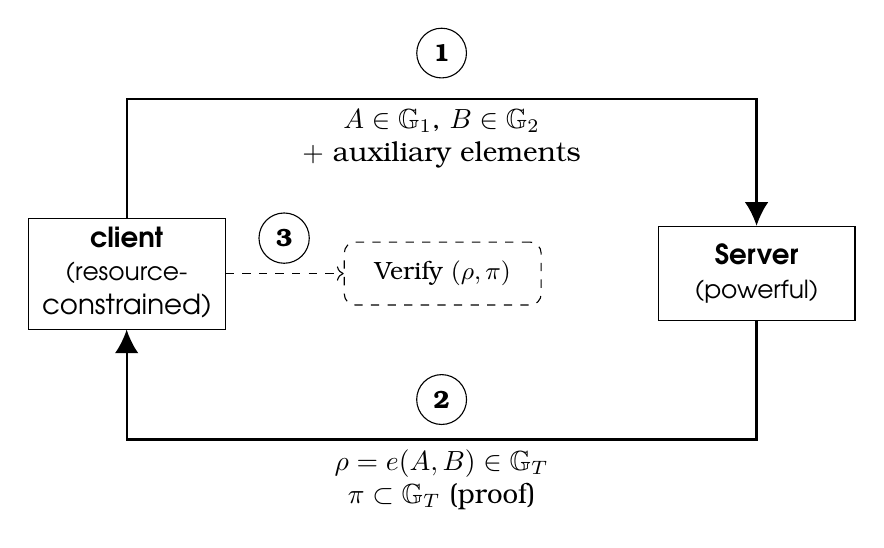
\begin{tikzpicture}[
    box/.style={rectangle, draw, minimum width=2.5cm, minimum height=1.2cm, align=center, font=\sffamily},
    arrow/.style={-{Latex[length=3mm,width=3mm]}, thick},
    stepnum/.style={circle, draw, fill=white, minimum size=0.5cm, font=\bfseries\small}
]
    % client and Server boxes
    \node[box] (client) at (0,0) {\textbf{client}\\\small(resource-\\constrained)};
    \node[box] (server) at (8,0) {\textbf{Server}\\\small(powerful)};
    
    % Arrows and labels with step numbers
    \draw[arrow] (client.north) -- ++(0,1.5) -| node[below, pos=0.25, align=center] {$A \in \Group_1$, $B \in \Group_2$\\$+$ auxiliary elements} (server.north);
    \node[stepnum] at (4,2.8) {1};
    
    \draw[arrow] (server.south) -- ++(0,-1.5) -| node[below, pos=0.25, align=center] {$\rho = e(A,B) \in \Group_T$\\$\pi \subset \Group_T$ (proof)} (client.south);
    \node[stepnum] at (4,-1.6) {2};
    
    % Verification box with step number
    \node[draw, dashed, rounded corners, minimum width=2.5cm, minimum height=0.8cm, right=1.5cm of client, align=center, font=\small] (verify) {Verify $(\rho,\pi)$};
    \draw[->, dashed] (client.east) -- (verify.west);
    \node[stepnum] at (2,0.45) {3};
\end{tikzpicture}
\caption{Flow diagram for \textbf{one-shot} pairing delegation.}
\label{fig:delegation-framework}
\end{figure}

\end{frame}

\begin{frame}
    \frametitle{Sequential Pairing Delegation}
    \begin{figure}[H]
\centering
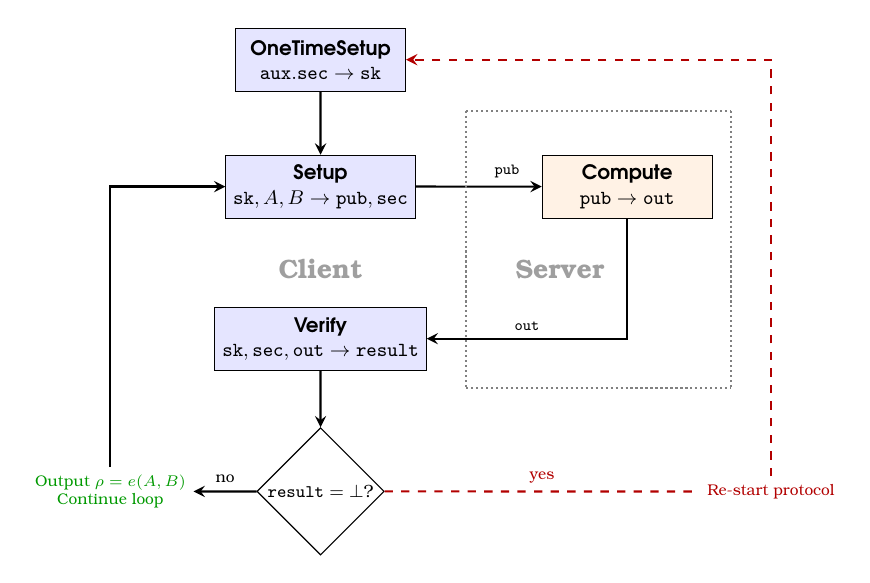
\begin{tikzpicture}[scale=0.8, every node/.style={transform shape},
    node distance=0.8cm and 2cm,
    box/.style={rectangle, draw, minimum width=2.7cm, minimum height=1cm, align=center, font=\small\sffamily},
    clientbox/.style={box, fill=blue!10},
    serverbox/.style={box, fill=orange!10},
    decision/.style={shape=diamond, draw, minimum width=1.5cm, minimum height=1.5cm, align=center, font=\footnotesize, inner sep=1pt},
    arrow/.style={->, >=stealth, thick},
    dasharrow/.style={->, >=stealth, thick, dashed},
    label/.style={font=\scriptsize, align=center}
]
    % OneTimeSetup (outside loop)
    \node[clientbox] (onetime) {\textbf{OneTimeSetup}\\$\auxsecpar \to \state$};
    
    % Loop start indicator
    % \node[below=0.8cm of onetime, label, text=red!70!black] (loopstart) {\textit{Sequential delegation loop}};
    
    % Setup phase
    \node[clientbox, below=1cm of onetime] (setup) {\textbf{Setup}\\$\state, A, B \to \pubvalue, \secvalue$};
    
    % Compute phase (Server)
    \node[serverbox, right=2cm of setup] (compute) {\textbf{Compute}\\$\pubvalue \to \serveroutput$};
    
    % Verify phase
    \node[clientbox, below=1.4cm of setup] (verify) {\textbf{Verify}\\$\state, \secvalue, \serveroutput \to \myresult$};
    
    % Result check decision
    \node[decision, below=0.9cm of verify] (result) {$\myresult = \bot$?};
    
    % Success output
    \node[left=1cm of result, label, text=green!60!black] (success) {Output $\rho=e(A,B)$\\Continue loop};
    
    % Failure output
    \node[right=5cm of result, label, text=red!70!black] (fail) {Re-start protocol};
    
    % Arrows
    \draw[arrow] (onetime) -- (setup);
    \draw[arrow] (setup) -- node[above, label, xshift=0.45cm] {$\pubvalue$} (compute);
    \draw[arrow] (compute.south) |- node[near end, above, label] {$\serveroutput$} (verify.east);
    \draw[arrow] (verify) -- (result);
    
    % Result decision paths
    \draw[arrow] (result) -- node[above, label] {no} (success);
    \draw[dasharrow, red!70!black, -] (result) -- node[above, label] {yes} (fail);
    
    % Loop back arrow (from success back to setup)
    \draw[arrow] (success) |- (setup.west);
    
    % Restart arrows (result yes and fail both go to onetime)
    % \draw[dasharrow, red!70!black] (result.west) -| node[near start, above, label, xshift=-0.3cm] {yes} ++(-1.5,0) |- (onetime.west);
    \draw[dasharrow, red!70!black] (fail.north) |- (onetime.east);
    
    % Client/Server separation line
    \draw[densely dotted, thick, gray] ($(setup.east)+(0.8,1.2)$) -- ($(setup.east)+(5,1.2)$);
    \draw[densely dotted, thick, gray] ($(setup.east)+(0.8,-3.2)$) -- ($(setup.east)+(5,-3.2)$);
    \draw[densely dotted, thick, gray] ($(setup.east)+(0.8,1.2)$) -- ($(setup.east)+(0.8,-3.2)$);
    \draw[densely dotted, thick, gray] ($(setup.east)+(5,1.2)$) -- ($(setup.east)+(5,-3.2)$);
    \node[label, gray!75] at ($(setup.south)+(0,-0.8)$) {\large\textbf{Client}};
    \node[label, gray!75] at ($(setup.south)+(3.8,-0.8)$) {\large\textbf{Server}};

\end{tikzpicture}
% \caption{\small Flow diagram for \textbf{sequential} pairing delegation.}
\label{fig:amore-flow}
\end{figure}

\end{frame}

\begin{frame}
    \frametitle{Delegation Properties}
\small
    \begin{itemize}
    \pause
	\item \textbf{Correctness}: If the \server behaves honestly, the output of the verification phase is the intended (vector of) pairing(s).	
\[	 
\myprob{\myresult=e(\AA,\BB)}{	(\pubvalue, \secvalue)\gets\onsetup(\state, {\AA},{\BB})\\
		 		\serveroutput\gets\compute(\pubvalue)\\
		 		\myresult\gets\onverify(\state,\secvalue,\serveroutput)}=1\,.
\]
\pause
	\item \textbf{Verifiability}: The \client must be able to detect with high probability when the \server returns an incorrect result.
\[	 
\myprob{\forge{\serveroutput}\gets\adversary\paren{\pubvalue}}{
		 		\forge{\serveroutput}\neq\serveroutput\\
		 		\onverify(\state,\secvalue,\serveroutput)\neq\bot}\leq\negl(\secpar)\,.
\]
\pause
	\item \textbf{Amortized Efficiency}: The \client's workload when delegating \totpairings pairings must be lower than computing them locally.
    \[
    \scalebox{0.9}{$\displaystyle
        \frac{\cost(\offsetup)+\totpairings\cdot\paren{\cost(\onsetup) + \cost(\onverify)}}{\totpairings}
        \leq \cost(e(A,B))$
    }
    \]
    \end{itemize}
\end{frame}

\begin{frame}
    \frametitle{One way to design this}
    \small
    \pause
    For \textbf{correctness} and \textbf{verifiability}: 
    \\
    \vspace{1em}
    \pause Construct a minimal verification equation in $\Group_T$ that relies on \client generated secrets for it to be satisfied. 
    \pause
    \\
    \vspace{1em}
    In particular, for public delegated inputs $(A,B)$ and generators $(P,Q,\gamma_T=e(P,Q))\in\Group_1\times\Group_2\times\Group_T$, 
    \begin{itemize}
        \setlength{\itemsep}{7.5pt}
        \pause
        \item generate secrets $(u,v,r)$, and set $\xi=\gamma_T^{-u\cdot v}=e([u]P,[-v]Q)=e(U,-V)$,
        \pause
        \item send $\pubvalue=(C,D)=([v](U+A),V-[\secexp]B)$,
        \pause
        \item request for $\serveroutput=(\rho,\gamma)=(e(A,B),e(A,D)\cdot e(C,Q))$,
        \pause
        \item and check $\left(\xi\overset{?}{=}\rho^{\secexp}\cdot\gamma\right)\wedge\left(\rho\overset{?}{\in}\Group_T\right)\,$.
    \end{itemize}
    \pause
    This guarantees unconditional security. Why?
\end{frame}

\begin{frame}
    \frametitle{One way to design this}
    \small
\begin{lemma}[Identifying forgeries]\label{lemma:sec-against-forgery}  
	Let \adversary be an algebraic adversary, $\paren{\xi,\secexp}\in\Group_T\times\Z_q^*$ the client's secret values, $\serveroutput=(\rho,\gamma)
	\in\Group_T\times\Group_T$ the output of an honest server, and \verify a verification phase consisting of the checks
	\begin{equation}
        \left(\xi\overset{?}{=}\rho^{\secexp}\cdot\gamma\right)\wedge\left(\rho\overset{?}{\in}\Group_T\right)\,.\label{eq:verif-eq}
    \end{equation}
    If $\paren{\adversary(\pubvalue)\to\forge{\serveroutput}\neq\serveroutput}\wedge\paren{\onverify(\forge{\serveroutput})\neq\bot}$ then \adversary outputs the secret \secexp.
\end{lemma}
\pause
\begin{proof}
    By the closure property of $\Group_T$,
    if $\paren{\xi=\paren{\forge{\rho}}^{\secexp}\cdot\paren{\forge{\gamma}}}\wedge\paren{\forge{\rho}\in\Group_T}$, then $\forge{\serveroutput}$ can be written as a deviation from the honest output: $\forge{\rho}=\rho\cdot\eta$ and $\forge{\gamma}=\gamma\cdot\eta^{-\secexp}$ for any public element $\eta\in\Group_T\,$. Indeed,  
    $\paren{\forge{\rho}}^{\secexp}\cdot\paren{\forge{\gamma}}
    =
    \paren{\rho\cdot\eta}^\secexp\cdot\gamma\cdot\eta^{-\secexp}=\rho^\secexp\cdot\gamma=\xi\,$.
\end{proof}
\end{frame}

\begin{frame}
    \frametitle{One way to design this}
    For \textbf{amortized efficiency}:
    \vspace{1em}
    \pause
    \begin{itemize}
        \setlength{\itemsep}{7.5pt}
        \item Sequential delegation: Reuse $\xi$ by generating in the next delegations secrets $(\secexp_i,u_i,v_i)$ such that $u_i\cdot v_i=u_j\cdot v_j\,$. The public values will still be equipped with an extra degree of freedom.  
        \pause
        \item Sample short scalars. Short $\Group_T$ exponentation is (a lot) cheaper than a full-range one.
        % \begin{align*}
        %     e(U_i,-V_i)=e(A_i,B_i)^{\secexp_i}\cdot e(A_i,V_i-[\secexp_i]B_i)\cdot e\left([v_i](U_i+A_i),\gentwo\right)
        % \end{align*}
    \end{itemize}
    \vspace{1em}
    \pause
    Wait a minute... do we still get unconditional security?
\end{frame}

\begin{frame}
    \frametitle{Meet-in-the-middle attack}
\small
\textbf{A toy example:}
\\
\vspace{1em}
Let $(\Group=\langle P\rangle,+)$ be a cyclic group of prime order $q$, 
% where $q$ is a $2\cdot\secpar$-bit integer, 
and $(\secexp_1,\secexp_2,u)$ a tuple of secret values such that 
$\secexp_1,\secexp_2\pick S\subset
\Z_q^*\,$ and $\varepsilon\pick\Z_q^*\,$. Let $\xi=[\varepsilon]P\in\Group\,$, and consider the public view 
	\begin{equation}
		\pubvalue=\begin{cases}
			\CC=[\secexp_1]\xi+\XX
			\\
			\DD=[\secexp_2]\xi+\YY
		\end{cases}\label{eq:toy-example-view}
		\,,
	\end{equation}
	where $\XX,\YY\in\Group$ are public and  $\XX\neq\CC,\YY\neq\DD$.  
    \adversary can attempt to learn the secret tuple from (\ref{eq:toy-example-view}) by picking an element 
	\begin{equation}
		\forge{\xi}\in\mathcal{I}=\left\{[t_1^{-1}](\CC-\XX)\colon t_1\in S\right\}\cap
		\left\{[t_2^{-1}](\DD-\YY)\colon t_2\in S\right\}
		\label{eq:intersection}		
	\end{equation}
	and its corresponding indexes $\forge{r}_1,\forge{r}_2\,$, 	
	which takes up to $2\cdot\size{S}$ computations.
\end{frame}

\begin{frame}
    \frametitle{Meet-in-the-middle attack}
    \begin{figure}[htbp]
\centering
\vspace{-1em}
\resizebox{\textwidth}{!}{%
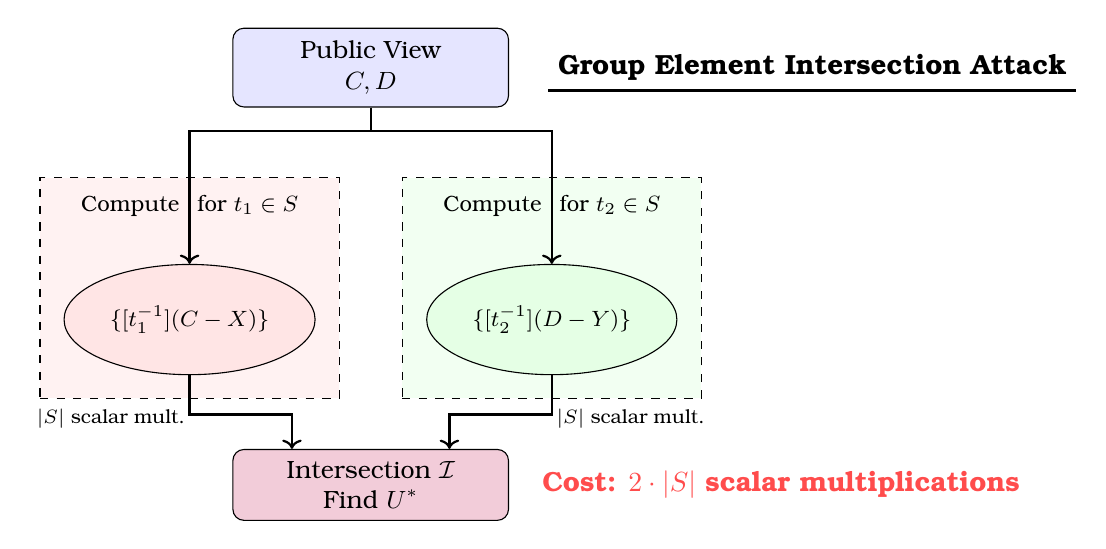
\begin{tikzpicture}[
    scale=1,
    node distance=1.2cm,
    box/.style={rectangle, draw, rounded corners, minimum width=3.5cm, minimum height=1cm, align=center, font=\small},
    arrow/.style={->, thick},
    label/.style={font=\footnotesize},
    computation/.style={rectangle, draw, dashed, minimum width=3.8cm, minimum height=2.8cm, align=center},
    set/.style={ellipse, draw, minimum width=3cm, minimum height=1.4cm, align=center, font=\footnotesize},
    decoration={brace}
]

% Group Element Intersection Attack

% Public view
\node[box, fill=blue!10] (pubview) at (0, 5) {Public View\\$\CC, \DD$};
\node[font=\bfseries, right=0.5cm of pubview] (title1) {Group Element Intersection Attack};
\draw[thick] (title1.south west) -- (title1.south east);

% Computation boxes
\node[computation, fill=red!5] (comp1) at (-2.3, 2.2) {};
\node[label, anchor=north] at (-2.3, 3.5) {Compute \,\,\,for $t_1\in S$};
\node[set, fill=red!10] (set1) at (-2.3, 1.8) {$\{[t_1^{-1}](\CC-\XX)\}$};
\node[label, below=0.3cm of set1, xshift=-1cm, font=\scriptsize] {$|S|$ scalar mult.};

\node[computation, fill=green!5] (comp2) at (2.3, 2.2) {};
\node[label, anchor=north] at (2.3, 3.5) {Compute \,\,\,for $t_2\in S$};
\node[set, fill=green!10] (set2) at (2.3, 1.8) {$\{[t_2^{-1}](\DD-\YY)\}$};
\node[label, below=0.3cm of set2, xshift=1cm, font=\scriptsize] {$|S|$ scalar mult.};

% Intersection
\node[box, fill=purple!20, minimum height=0.9cm] (intersection1) at (0, -0.3) {Intersection $\mathcal{I}$\\Find $\forge{U}$};

% Arrows
\draw[arrow] (pubview.south) -- ++(0,-0.3) -| (set1.north);
\draw[arrow] (pubview.south) -- ++(0,-0.3) -| (set2.north);
\draw[arrow] (set1.south) -- ++(0,-0.5) -| ([xshift=-1cm]intersection1.north);
\draw[arrow] (set2.south) -- ++(0,-0.5) -| ([xshift=1cm]intersection1.north);

% Cost label
\node[label, font=\bfseries, text=red!70, right=0.3cm of intersection1] {Cost: $2\cdot|S|$ scalar multiplications};

\end{tikzpicture}%
}
\vspace{0.5em}
% \caption{\small Analogy between the intersection attack on partially-masking secret variables (above) and Diffie-Hellman's meet-in-the-middle attack (below) on Double DES encryption (adapted from \cite{diffiehellman-mitm}).}
\label{fig:meet-in-the-middle}
\end{figure}
\end{frame}

\begin{frame}
    \frametitle{Meet-in-the-middle attack}
    \begin{figure}[htbp]
\centering
\vspace{-1em}
\resizebox{\textwidth}{!}{%
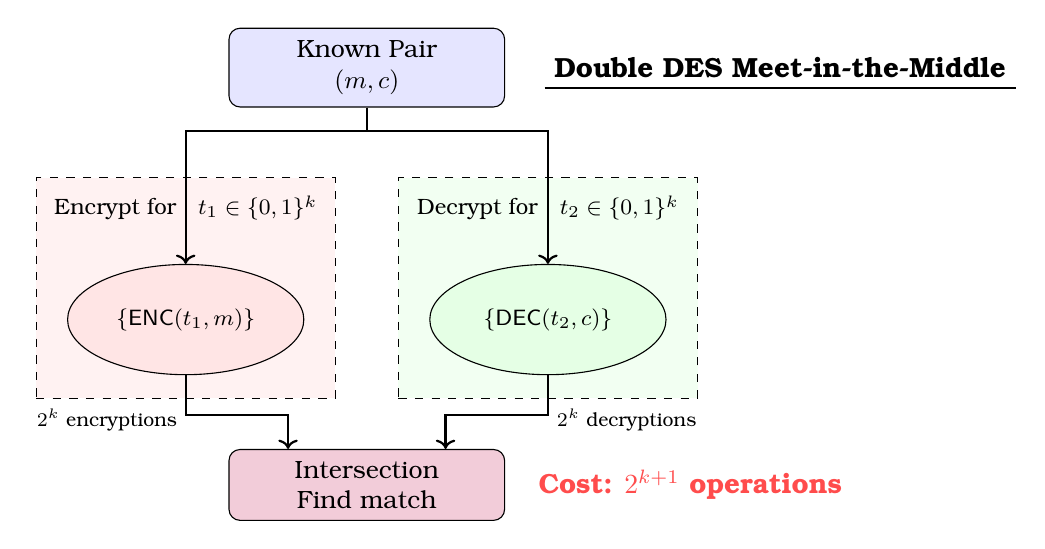
\begin{tikzpicture}[
    scale=1,
    node distance=1.2cm,
    box/.style={rectangle, draw, rounded corners, minimum width=3.5cm, minimum height=1cm, align=center, font=\small},
    arrow/.style={->, thick},
    label/.style={font=\footnotesize},
    computation/.style={rectangle, draw, dashed, minimum width=3.8cm, minimum height=2.8cm, align=center},
    set/.style={ellipse, draw, minimum width=3cm, minimum height=1.4cm, align=center, font=\footnotesize},
    decoration={brace}
]
% Bottom section: Double DES Meet-in-the-Middle

% Plaintext-ciphertext pair
\node[box, fill=blue!10] (pair) at (0, -4.8) {Known Pair\\$(m, c)$};
\node[font=\bfseries, right=0.5cm of pair] (title2) {Double DES Meet-in-the-Middle};
\draw[thick] (title2.south west) -- (title2.south east);

% Computation boxes
\node[computation, fill=red!5] (comp3) at (-2.3, -7.6) {};
\node[label, anchor=north] at (-2.3, -6.3) {Encrypt for \,\,\,\,$t_1\in\{0,1\}^k$};
\node[set, fill=red!10] (set3) at (-2.3, -8) {$\{\enc(t_1,m)\}$};
\node[label, below=0.3cm of set3, xshift=-1cm, font=\scriptsize] {$2^k$ encryptions};

\node[computation, fill=green!5] (comp4) at (2.3, -7.6) {};
\node[label, anchor=north] at (2.3, -6.3) {Decrypt for \,\,\,\,$t_2\in\{0,1\}^k$};
\node[set, fill=green!10] (set4) at (2.3, -8) {$\{\dec(t_2,c)\}$};
\node[label, below=0.3cm of set4, xshift=1cm, font=\scriptsize] {$2^k$ decryptions};

% Intersection
\node[box, fill=purple!20, minimum height=0.9cm] (intersection2) at (0, -10.1) {Intersection\\Find match};

% Arrows
\draw[arrow] (pair.south) -- ++(0,-0.3) -| (set3.north);
\draw[arrow] (pair.south) -- ++(0,-0.3) -| (set4.north);
\draw[arrow] (set3.south) -- ++(0,-0.5) -| ([xshift=-1cm]intersection2.north);
\draw[arrow] (set4.south) -- ++(0,-0.5) -| ([xshift=1cm]intersection2.north);

% Cost label
\node[label, font=\bfseries, text=red!70, right=0.3cm of intersection2] {Cost: $2^{k+1}$ operations};

\end{tikzpicture}%
}
\vspace{0.5em}
% \caption{\small Analogy between the intersection attack on partially-masking secret variables (above) and Diffie-Hellman's meet-in-the-middle attack (below) on Double DES encryption (adapted from \cite{diffiehellman-mitm}).}
\label{fig:meet-in-the-middle2}
\end{figure}

\end{frame}

\begin{frame}
    \frametitle{What now?}
    \small
    \pause
    If short scalars are not used, minimal efficiency is gained. If short scalars are used, no unconditional security can be proven... 
    \\
    \pause
    \vspace{1em}
    \textbf{Remark}: Once the protocol execution is finished, \adversary can no longer cheat. We could aim for everlasting security instead.
    \\
    \pause
    \vspace{1em}
    \textbf{(Unorthodox) Solution}: 
    \pause
    \begin{itemize}
        \item Add a timeout parameter to the protocol.
        \pause
        \item Bound \adversary computationally... but not in the conventional way: Assume \adversary is not more powerful than the entire Bitcoin network, i.e., \adversary is allowed to compute $2^\kappa$ scalar group multiplications per second ($\kappa$ matching the current hashrate conversion).
    \end{itemize}  
\end{frame}


\begin{frame}
    \frametitle{Adversary winning probability}
    \small
    \pause
    \textbf{Time-bound}: \adversary computes $\leq 2^\kappa$ short exponentations in $\timepar$ seconds.
    \pause
    \\
    \textbf{Best strategy}: Choose $S_1,S_2\subset\range{2^\effpar}\colon\size{S_1}+\size{S_2}\leq 2^\kappa$ and intersect sets.
    \pause
    \begin{align*}
        &\myprob{\forge{\serveroutput}\gets\adversary\paren{\pubvalue}}{
                        \forge{\serveroutput}\neq\serveroutput\\
                        \onverify(\state,\secvalue,\serveroutput)\neq\bot}
        \\[10pt]
        \pause
        \leq&\myprobNoBar{\xi\in\begin{array}{c}
            \mathrm{set}\ \{[r^{-1}](C-X):\ r\in S_1\}\\[2pt]
            \cap\\[2pt]
            \mathrm{set}\ \{[r^{-1}](D-Y):\ r\in S_2\}
            \end{array}}
            \\[10pt]
            \pause
        \leq&\myprobNoBar{\begin{array}{c}
            \mathrm{event}\ \{r_1\in S_1\}\\[2pt]
            \wedge\\[2pt]
            \mathrm{event}\ \{r_2\in S_2\}
            \end{array}}
        \leq 2^{-\statsecpar}~~~\text{ if } \effpar=\lceil\frac{\statsecpar-1}{2}+\kappa\rceil
    \end{align*}

\end{frame}

\begin{frame}
    \frametitle{Performance results}
    \begin{figure}[!htb]
\centering
\resizebox{0.7\textwidth}{!}{%
\begin{tikzpicture}
    % Row 1: M=3
    % Label for M=3
    \node[font=\small\bfseries, anchor=west] at (-2.5, 1) {$\batchsize=3$};
    
    % BLS12-381 (M=3)
    \begin{axis}[
        name=plot4,
        width=0.32\textwidth,
        height=4.75cm,
        title={BLS12-381},
        title style={font=\small, yshift=0.2cm},
        ylabel style={font=\small},
        yticklabel style={font=\tiny},
        xtick=\empty,
        enlarge x limits=0.25,
        ymin=0, ymax=2000,
        ymajorgrids=true,
        grid style=dashed,
    ]
    \addplot[ybar,pattern=north west lines,pattern color=black!50,bar width=8pt] coordinates {(1,1470)};
    \addplot[ybar,pattern=dots,pattern color=gray!60,bar width=8pt] coordinates {(2,1499)};
    \addplot[ybar,pattern=horizontal lines,pattern color=blue!60,bar width=8pt] coordinates {(3,1324)};
    \addplot[ybar,pattern=crosshatch,pattern color=orange!60,bar width=8pt] coordinates {(4,598)};
    \end{axis}

    % BLS24-509 (M=3)
    \begin{axis}[
        name=plot5,
        at={(plot4.east)},
        anchor=west,
        xshift=0.75cm,
        width=0.32\textwidth,
        height=4.75cm,
        title={BLS24-509},
        title style={font=\small, yshift=0.2cm},
        yticklabel style={font=\tiny},
        xtick=\empty,
        enlarge x limits=0.25,
        ymin=0, ymax=11000,
        ymajorgrids=true,
        grid style=dashed,
    ]
    \addplot[ybar,pattern=north west lines,pattern color=black!50,bar width=8pt] coordinates {(1,7591)};
    \addplot[ybar,pattern=dots,pattern color=gray!60,bar width=8pt] coordinates {(2,8959)};
    \addplot[ybar,pattern=horizontal lines,pattern color=blue!60,bar width=8pt] coordinates {(3,7551)};
    \addplot[ybar,pattern=crosshatch,pattern color=orange!60,bar width=8pt] coordinates {(4,3469)};
    \end{axis}

    % BLS48-575 (M=3)
    \begin{axis}[
        name=plot6,
        at={(plot5.east)},
        anchor=west,
        xshift=0.75cm,
        width=0.32\textwidth,
        height=4.75cm,
        title={BLS48-575},
        title style={font=\small, yshift=0.2cm},
        yticklabel style={font=\tiny},
        xtick=\empty,
        enlarge x limits=0.25,
        ymin=0, ymax=45000,
        ymajorgrids=true,
        grid style=dashed,
    ]
    \addplot[ybar,pattern=north west lines,pattern color=black!50,bar width=8pt] coordinates {(1,36688)};
    \addplot[ybar,pattern=dots,pattern color=gray!60,bar width=8pt] coordinates {(2,36696)};
    \addplot[ybar,pattern=horizontal lines,pattern color=blue!60,bar width=8pt] coordinates {(3,31339)};
    \addplot[ybar,pattern=crosshatch,pattern color=orange!60,bar width=8pt] coordinates {(4,13016)};
    \end{axis}

    % Row 2: M=10
    % Label for M=10
    \node[font=\small\bfseries, anchor=west] at (-2.5, -2) {$\batchsize=10$};
    
    % BLS12-381 (M=10)
    \begin{axis}[
        name=plot7,
        at={(plot4.south)},
        anchor=north,
        yshift=-1cm,
        width=0.32\textwidth,
        height=4.75cm,
        ylabel style={font=\small},
        yticklabel style={font=\tiny},
        xtick=\empty,
        enlarge x limits=0.25,
        ymin=0, ymax=2000,
        ymajorgrids=true,
        grid style=dashed,
    ]
    \addplot[ybar,pattern=north west lines,pattern color=black!50,bar width=8pt] coordinates {(1,1470)};
    \addplot[ybar,pattern=dots,pattern color=gray!60,bar width=8pt] coordinates {(2,1113)};
    \addplot[ybar,pattern=horizontal lines,pattern color=blue!60,bar width=8pt] coordinates {(3,922)};
    \addplot[ybar,pattern=crosshatch,pattern color=orange!60,bar width=8pt] coordinates {(4,427)};
    \end{axis}

    % BLS24-509 (M=10)
    \begin{axis}[
        name=plot8,
        at={(plot7.east)},
        anchor=west,
        xshift=0.75cm,
        width=0.32\textwidth,
        height=4.75cm,
        yticklabel style={font=\tiny},
        xtick=\empty,
        enlarge x limits=0.25,
        ymin=0, ymax=10000,
        ymajorgrids=true,
        grid style=dashed,
    ]
    \addplot[ybar,pattern=north west lines,pattern color=black!50,bar width=8pt] coordinates {(1,7591)};
    \addplot[ybar,pattern=dots,pattern color=gray!60,bar width=8pt] coordinates {(2,6724)};
    \addplot[ybar,pattern=horizontal lines,pattern color=blue!60,bar width=8pt] coordinates {(3,5274)};
    \addplot[ybar,pattern=crosshatch,pattern color=orange!60,bar width=8pt] coordinates {(4,2308)};
    \end{axis}

    % BLS48-575 (M=10)
    \begin{axis}[
        name=plot9,
        at={(plot8.east)},
        anchor=west,
        xshift=0.75cm,
        width=0.32\textwidth,
        height=4.75cm,
        yticklabel style={font=\tiny},
        xtick=\empty,
        enlarge x limits=0.25,
        ymin=0, ymax=45000,
        ymajorgrids=true,
        grid style=dashed,
    ]
    \addplot[ybar,pattern=north west lines,pattern color=black!50,bar width=8pt] coordinates {(1,36688)};
    \addplot[ybar,pattern=dots,pattern color=gray!60,bar width=8pt] coordinates {(2,26028)};
    \addplot[ybar,pattern=horizontal lines,pattern color=blue!60,bar width=8pt] coordinates {(3,20605)};
    \addplot[ybar,pattern=crosshatch,pattern color=orange!60,bar width=8pt] coordinates {(4,8467)};
    \end{axis}

    % Legend
    \node[draw, rounded corners, rectangle, below=0.5cm of plot7.south, xshift=2.5cm] {
        \begin{tikzpicture}
            \node[rectangle, pattern=north west lines, pattern color=black!50, draw, minimum width=0.3cm, minimum height=0.3cm] (box1) at (0,-0.3) {};
            \node[anchor=west, yshift=0pt, align=left] at (box1.east) {\small Pairing};
            
            \node[rectangle, pattern=dots,pattern color=gray!60, draw, minimum width=0.3cm, minimum height=0.3cm] (box2) at (2.5,-0.3) {};
            \node[anchor=west, yshift=0pt, align=left] at (box2.east) {\small MV19};
            
            \node[rectangle, pattern=horizontal lines,pattern color=blue!60, draw, minimum width=0.3cm, minimum height=0.3cm] (box3) at (5.0,-0.3) {};
            \node[anchor=west, yshift=0pt, align=left] at (box3.east) {\small CKC23};
            
            \node[rectangle, pattern=crosshatch,pattern color=orange!60, draw, minimum width=0.3cm, minimum height=0.3cm] (box4) at (7.5,-0.3) {};
            \node[anchor=west, yshift=0pt, align=left] at (box4.east) {\small AmorE};
            
        \end{tikzpicture}
    };
\end{tikzpicture}
}
% \caption{\small Batch pairing delegation cost comparison for type \pvpv.}
\label{fig:batch-pvpv-comparison}
\end{figure}

\end{frame}

\begin{frame}
    \begin{center}
    
    Thank you for your attention :)
        \\
        \vspace{3em}
    Paper: eprint.iacr.org/2025/542        
    \end{center}

\end{frame}
% \begin{frame}
% 	\begin{align*}
% 		\rho^\secexp\cdot \gamma & = e(A,B)^\secexp\cdot \left(e(A,D)\cdot e(C,\gentwo)\right) 
% 		\\[0.3em]
% 		% \displaybreak[1]
% 		&=e(A,[\secexp]B)\cdot e(A,V-[\secexp]B)\cdot e\left([-\longtermsecret\cdot u^{-1}](U+A),\gentwo\right)
% 		\\[0.3em]
% 		% \displaybreak[1]
% 		& = e(A,V)\cdot e(U+A,[-\longtermsecret\cdot u^{-1}]\gentwo)
% 		\\[0.3em]
% 		% \displaybreak[1]
% 		& = e(A,V)\cdot e(U+A,-V)
% 		\\[0.3em]
% 		% \displaybreak[1]
% 		& = e(U,-V)=e(\genone,\gentwo)^{u\cdot (-\longtermsecret)\cdot u^{-1}}=\gentt^{-\longtermsecret}=\xi
% 	\end{align*}
% \end{frame}

\end{document}